%%%%%%%%%%%%%%%%%%%%%%%%%%%%%%%%%%%%%%%%%%%%%%%%%%%%%%%%%%%%%%%%%
\chapter{Numerical Operations} 
%%%%%%%%%%%%%%%%%%%%%%%%%%%%%%%%%%%%%%%%%%%%%%%%%%%%%%%%%%%%%%%%%

%-------------------------------------
\section{Bits, Bytes, and Floating Point}
%-------------------------------------
Computers have a finite number of ways to represent numbers. That is, they can only approximate a small subset of real numbers. Understanding this is an essential component of conducting numerical operations: You need to understand how and why numerical errors accumulate, and when they interfere with a calculation. 

The unit of computing representation is a \textbf{bit} (unit represented by b), i.e. a circuit that is either open or closed.  Eight bits are grouped into one \textbf{byte} (unit represented by B), as shown in Figure \ref{fig:Byte}. This number evolved from computer architectures in the early days of computing, and was first standardized by  ISO/IEC 2382-1:1993.  In one byte, positions go from 0 to 7, usually represented from right to left. A 1 in the first position represents $2^0$, in the second position is $2^1$, and so on. 

\begin{figure}[h]\label{fig:Byte}
	\centering
		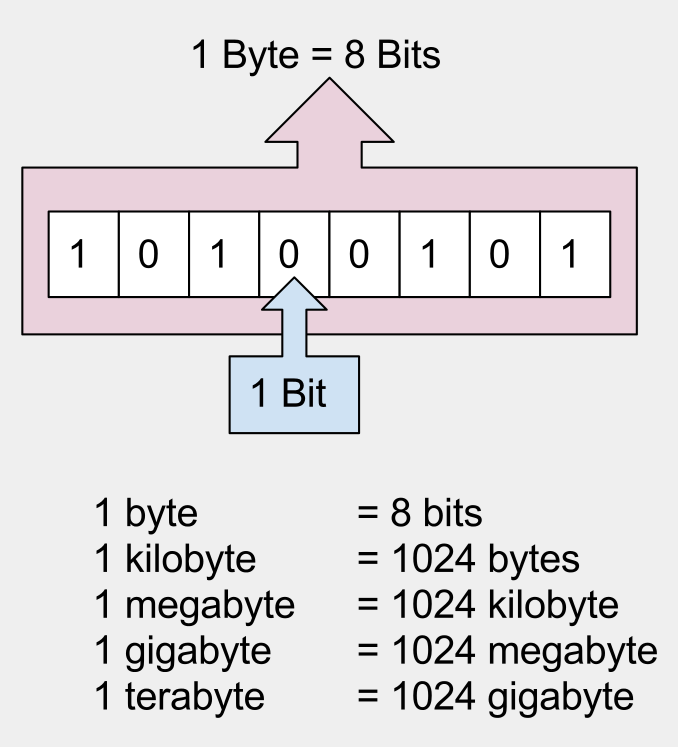
\includegraphics[width=0.5\textwidth]{../images/ChapterNumericalOps/Byte.png} 
	\caption{Bits and Bytes \cite{wiki:Byte}. Reading from left to right, the example represents: $2^0 + 2^2 + 2^5 + 2^7 = 1 +  4 + 32 + 128= 165$. If you read from right to left (this is the standard way to represent bits), you  would obtain  $2^0 + 2^2 + 2^5 + 2^7 = 165$. In this case, left-to-right and right-to-left produce the same result. But in general they don't have to be the same. What happens if you replace any zero with a one, and compute both directions again? Thus, representation matters, and you need to know the convention.}
	\label{fig:Byte}
\end{figure}

A naive way to represent numbers with a computer is to allocate $N$ decimal digits, for each number. For example: 
{\ttfamily\[
	012.345
\]}
This example  represents a 6-digit fixed-point system. This 6-digit fixed-point system results in errors in some sum cases: 
{\ttfamily\[
	999.999 + 999.999 = \text{OVERFLOW}
\]}
Also errors occur in multiplication and division
{\ttfamily\[
	013.000 / 003.000 = 004.333
\]}
In this case, we lose all digits after the third decimal. 

We can allow the decimal point to ``float'' to gain accuracy with the same number of digits. For example: 	
{\ttfamily\[
	013.000 / 003.000 = 4.33333
\]}
We could even represent larger numbers than 6 digits allowed us before: 
{\ttfamily\[
	999.999 \times 999.999 = 9.99998 \times 10^5
\]}

%-------------------------------------
\subsection{The IEEE Standard for Floating-Point Arithmetic}
%-------------------------------------
The IEEE Standard for Floating-Point Arithmetic (IEEE 754) is a technical standard for 	floating-point computation established in 1985 by the Institute of Electrical and 	Electronics Engineers (IEEE). 
	\begin{itemize}
		\item Finite numbers may be either base 2 (binary) or base 10 (decimal). 
		\item Each finite number is described by three integers: 
					\begin{enumerate}
						\item $s$ = a sign (zero or one), 
						\item $c$ = a significand (or `coefficient'), 
						\item $q$ = an exponent. 
					\end{enumerate}
		\item The numerical value of a finite number is $(-1)^s \times c \times bq$ where b is the base (2 or 10), also called radix. 
	\end{itemize}

The three fields in an IEEE-754 float. Binary floating-point numbers are stored in a sign-magnitude form where the most significant bit is the \textit{sign} bit, \textit{exponent} is the biased exponent, and \textit{fraction} is the significand minus the most significant bit. Figure \ref{fig:32bit} shows a 32-bit number, also known as a single-precision floating number, whereas Figure \ref{fig:64bit} depitcs a 64-bit number, also known as double-precision floating number. 

\begin{figure}
	\centering
		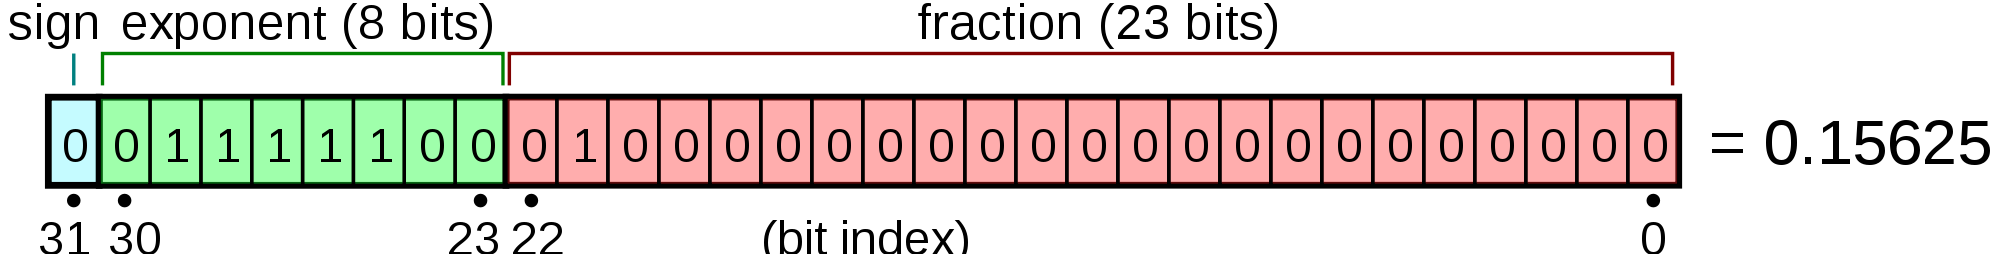
\includegraphics[width=4in]{../images/ChapterNumericalOps/Single_Floating_Point_Format.png}
		\caption{Representation of a single precision number \cite{wiki:SinglePrec}}
		\label{fig:32bit}
\end{figure}
	
\begin{figure} 
	\centering
		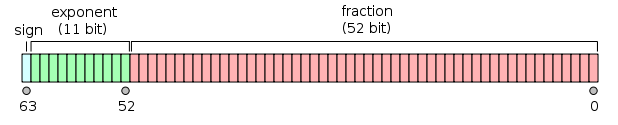
\includegraphics[width=4in]{../images/ChapterNumericalOps/Double_Floating_Point_Format.png}
		\caption{Representation of a double precision number \cite{wiki:DoublePrec}.}
		\label{fig:64bit}
\end{figure}	

If we want to represent a real number with a finite number $N$ of memory positions, we can reserve one position for the sign, $N-k-1$ for the integer part, and $k$ for the digits beyond the separator or fractional part. The notation conventionally adopted is \cite{quarteroni2010numerical}:
\begin{equation}\label{eq:Floating}
	x = (-1)^s[a_{N-2}a_{N-3}...a_{k}.a_{k-1}a_{k-2}...a_{0}]  = (-1)^s \cdot \beta^{-k} \sum_{j=0}^{N-2}a_j \beta^j
\end{equation}
where $\beta$ is the base of the representation (it could be any number, but usually it is $2$ or $10$), $s$ is either 1 or 0,  $N$ is the number of digits in the significand,  $a_j$ is the $j^{th}$ digit, $k$ is the exponent. 

The floating point representation in equation \ref{eq:Floating} limits the minimum or maximum number unless some scaling is allowed. In such case, a \textit{floating point} representation is given by 
\begin{equation}\label{eq:Normalized}
	x = (-1)^s \cdot [0.a_{1}a_{2}...a_{t}] \cdot  \beta^{e} = (-1)^s \cdot m  \cdot \beta^{e-t}
\end{equation}
where $t \in \mathbb{N}$ is the number of significant digits $a_i$ with $0 \leq a_i \leq \beta - 1$, $m=a_{1}a_{2}...a_{t}$ is an integer number called \textit{mantissa}
with $0 \leq m \leq \beta^t-1$ and $e$ is an integer number called \textit{exponent} with $L \leq e \leq U$ (typically $L \leq 0$ and $U \geq 0$). If we require $a_1 \neq 0$ and $m \geq \beta^{t-1}$ then the representation in equation \ref{eq:Normalized} is called \textit{normalized}.

%It is important to understand the context in which the word \textit{mantissa} is used.  The word \textit{mantissa} in computer science  is defined as the part of a floating-point number representing the significant digits of that number multiplied by the base raised to the exponent to give the actual value of the number; it is often used as a synonym for \textit{significand}. This, however, departs from the historical mathematical tradition because \textit{mantissa} was first defined as the part after the separator (or fractional part) of a logarithm. Thus, in mathematics, a \textit{mantissa} is the logarithm of a \textit{significand}.  }

The term \textit{mantissa} in computer science commonly refers to the significant digits of a floating-point number, essentially synonymous with \textit{significand}. This usage diverges from its historical mathematical meaning, where \textit{mantissa} denoted the fractional part of a logarithm. Notably, among the many authors that followed John Napier's early logarithmic work, ``\textit{Mirifici Logarithmorum Canonis Descriptio}" (1614) \cite{napier1614mirifici}, it was John Wallis who used the word ``\textit{appendage}''  in the English version of ``\textit{A Treatise of Algebra},'' \cite[p. 38]{wallis1685proposal} (1658),  translated into Latin as ``manti\hspace{-0.03in}$\int$\hspace{-0.06in}$\int$\hspace{-0.03in}am'' (in modern form \textit{mantissa}) \cite[p. 41]{wallis1693opera} (1681) (see Figure \ref{fig:Mantissam}), to describe the decimal part of a logarithm, not the logarithm of a significand. This distinction highlights the evolution of mathematical terminology over time.  

\begin{figure} 
	\centering
		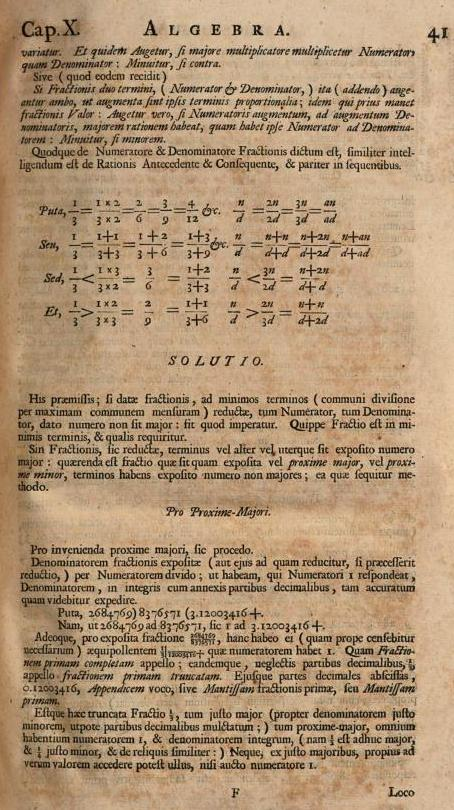
\includegraphics[width=5in]{../images/ChapterNumericalOps/Mantissam.jpg}
		\caption{Page 41 of ``\textit{A Treatise of Algebra},'' , where the word mantissa is introduced. J. Wallis. \textit{Opera mathematica: De Algebra Tractatus}. Number v. 5 Anno 1685 Anglice editus; Nunc Auctus Latine. Theatrum Sheldonianum, 1693.}
		\label{fig:Mantissam}
\end{figure}	





%The total number of normalized floating point numbers of a double precision number $\mathbb{F}$ that can be represented with the IEEE standard is given by equation \ref{eq:CardinalityDouble}:
%\begin{eqnarray}
%	card \mathbb{F} & = & 2(\beta-1)\beta^{t-1}(U-L+1) + 1 \label{eq:CardinalityDouble} \\
%					& = & 2(2-1)2^{52-1}(1023-(-1022)+1) + 1 \nonumber \\
%					& = & 9.214 \times 10^{18} \nonumber
%\end{eqnarray}

%We can approximate this value by noticing that a double precision number is represented by 64 bits, starting from zero. Therefore, 
%\[
%	card \mathbb{F} \approx 2^{63} \approx 9.223 \times 10^{18}
%\]

%A better approximation results invariably in equation \ref{eq:CardinalityDouble}.

	
%-------------------------------------
\subsection{A Bestiary of Floating Point Anomalies}\label{sec:FloatingPoint}
%-------------------------------------

One of the most surprising aspects of floating-point arithmetic is that simple operations do not result in expected results. For instance, the addition $1-1/3-2/3$ results algebraically in zero. However,  
{\ttfamily\[
	1-1/3-2/3 = 1.1102e-16, 
\]}	{\ttfamily\[		
	1-2/3-1/3 = 5.5511e-17.		
\]}
Thus, not only the operation is not zero, but also the order of summands matter, i.e. floating point addition is not commutative. Hence,  $1-1/3-2/3 \neq 1-2/3-1/3 \neq 0$

Because floating point numbers cannot represent all real numbers, errors of representation occur in many cases. But why is the operation noncommutative?  \QA %Come back to this question to provide a technical answer after you read  Section \ref{sec:FloatingPoint}. 

The following instruction compares whether $10^{30} + 1 - 10^{30}$ equals the value 1. Using elementary arithmetic, the answer should be a resounding \textit{yes}. In the Python language, the exponent is represented by a double asterisk, like in Fortran, instead of the carat sign (\^{}) used in most other computing platforms. The double equal sign tests whether the two sides are equal, and returns a Boolean value of \textit{true} or \textit{false}. Hence, the question is translated into the following instruction: 

\begin{lstlisting}[language=Python]
	10**30 + 1 - 10**30 == 1   
\end{lstlisting}

This particular instruction  returns a Boolean value of \textit{true} in Python and \textit{false} in Matlab (the correct Matlab syntax is $10\hat{\phantom{.}}30 + 1 - 10\hat{\phantom{.}}30 == 1$). However, the following statement:  

\begin{lstlisting}[language=Python]
	10**30 + 1. - 10**30 == 1
\end{lstlisting}

\noindent returns \textit{false} in Python. Why? \QA 

An operation like 

\begin{lstlisting}[language=Python]
	10**20 + 1 - 10**20 == 1
\end{lstlisting}

\noindent returns different results in Matlab, C, Fortran (\textit{false}) vs. Python (\textit{true}). It might be tempting to declare Python the winner in numerical computation, but what truly happens is that Python does not follow the IEEE-754 standard strictly. To learn about more subtleties of floating point in Python, go to \url{https://docs.python.org/3/tutorial/floatingpoint.html} In most cases, deviations from the standard in the Python interpreter are harmless and have an ideological origin rather than a technical one. However, it is conceivable that extreme algorithms developed under the IEEE standard would have to be carefully adapted in Python. There are alternatives, but they are beyond the scope of this chapter. For now, it suffices to say that there are landmines in the Python landscape. 
	
We can explore further discrepancies in extreme floating point values by exploring in two numerical environments the results of $10\cdot 10^b + 1 - 10\cdot 10^b$ for different values of $b$. Download and install Python, Matlab, R, or compile a C/C++ program that executes the same operations. Compare what happens in these environments when you choose $b \in \{10, 1e2, 1e10, 1e100, 1e1000\}$. Describe  the discrepancies, and analyze. \QA



%-----------------------------------------
\section{Introduction to NumPy}
%-----------------------------------------

To execute mathematical operations beyond basic operations with real numbers, you need to import a numerical library. Matrix operations are executed through functions in NumPy. Hence, the first step is to load NumPy. 

\begin{lstlisting}[language=Python]
In : import numpy as np
\end{lstlisting}

The library NumPy offers easy access to commonly used constants, such as:

\vs 

\begin{tabular}{r|l}
Constant 			& Value\\
\hline
np.e 				& Returns the number $e$ \\
np.pi 			& Returns the number $\pi$ \\
np.inf 			& Returns the number $\infty$ \\
np.nan 			& NaN, not-a-number \\
\hline
\end{tabular}

\vs

%MATLAB: Infinity is generated by dividing a nonzero value by zero, or by
%evaluating well defined mathematical expressions that overflow.
%(Try $10^{310}$ or $\exp(999)$.)

%MATLAB: Not-a-number is generated by trying to evaluate expressions like
%0/0 or Inf-Inf that do not have well defined mathematical values.

With NumPy, we can now access commonly used mathematical functions. Among others: \vs

\begin{tabular}{r|l}
Function 			& Operation \\
\hline
np.abs(x)   		& Absolute value $|x|$ \\
np.sqrt(x)			&  Square root $\sqrt{x}$ \\
np.exp(x) 			& Exponential function $e^x$ \\
np.log(x) 			& $\log(x)$ where $x$ is positive real number\\
np.sin(x)			&  $\sin(x)$ where $x$ is assumed to be in radians \\
np.cos(x) 			& $\cos(x)$ where $x$ is assumed to be in radians \\
\hline
\end{tabular}

\vs 
Expressions use the arithmetic operators and precedence rules you already know by now.
There are also functions, such as cosine or sine. You surround the
input to the function by parenthesis. For example, to calculate the
square root of two, you type

\begin{lstlisting}[language=Python]
In 	: np.sqrt(2)
Out	: 1.4142135623730951
\end{lstlisting}

However, you cannot use the function {\s sqrt} with negative numbers. What would you have to do to alloy Python to compute the square root of a negative number and return a complex number? \QA  %So, instead of {\s sqrt(-2)} you will have to use {\s (-2)**0.5}. 

The library NumPy has \textit{many} functions. A comprehensive list can be found at \url{https://numpy.org/doc/stable/reference/}. You will observe that immediately below the command you entered, the prompt will show {\s Out[n]: 3.0}, where {\s n} stands for the command sequence number (recall, the first executed command has $n=1$, the second $n=2$, and so on).

Now enter the following command: 

\begin{lstlisting}[language=Python]
	x = np.random.standard_normal(3)  
\end{lstlisting}

There is no output. Why do you think this is the behavior? \QA On the right-hand side of the Spyder window there is a tab called \textit{Variable Explorer}. It will show the value of $x$. Alternatively, you can enter 

\begin{lstlisting}[language=Python]
	print(x)
\end{lstlisting}

Alternatively, you can print the result directly without assigning it to a variable. Try

\begin{lstlisting}[language=Python]
	print(np.random.standard_normal(3))
\end{lstlisting}

Why are the results of this last operation different to the values stored in variable $x$? \QA



%-----------------------------------------
\subsection{Matrix Operations}
%-----------------------------------------

The basic data element in NumPy is a multi-dimensional array. 
Special meaning is sometimes attached to 1-by-1 matrices, which are
called scalars, and to matrices with only one row or column, which
are called vectors. Python has other ways of storing both numeric
and non-numeric data, but in the beginning, it is usually best to
think of everything as a matrix.

Row vectors are delimited in notation by square brackets. A comma separates individual numbers in a row vector. Multiple row vectors of the same size are separated by commas, and are delimited by square brackets to define a matrix. It is common practice to use a capital letter when naming matrices in order to distinguish them from a single vector, scalar or variable value. 

Now, we will create a vector and a matrix to demonstrate simple matrix operations \vs

\begin{tabular}{r|l}
Function 			& Operation \\
\hline
$x = np.array([1,2,3,4])$ 					&   Creates the row vector $\x = [1,2,3,4]$\\
$b = np.array([1,2,3])$ 					&   Creates the row vector $\bb = [1,2,3]$\\
$A = np.array([[1,2,3], [4,5,6], [7,8,9]])$  &   Creates the matrix $ A = \begin{bmatrix} 1 & 2 & 3\\ 4 & 5 & 6 \\ 7 & 8 & 9 \end{bmatrix} $\\
$B = np.ones([2,3])$   &   Creates the matrix $ A = \begin{bmatrix} 1 & 1 & 1\\ 1 & 1 & 1 \end{bmatrix} $\\
$C = np.zeros([2,3])$   &   Creates the matrix $ A = \begin{bmatrix} 0 & 0 & 0\\ 0 & 0 & 0 \end{bmatrix} $\\
\hline
\end{tabular}

\vs
The following commands demonstrate basic vector manipulation cases:
\vs

\begin{tabular}{r|l}
Operation 			& Outcome \\
\hline
$x[-1]$ 				&   Returns 4, the last element of $x$\\
$x[1]$ 					&   Returns 2, the second element of $x$\\
$x[-2]$ 				&  Returns 3, the second to last element of $x$\\
\hline
\end{tabular}

\vs
The colon (:) operator is notable. In vector notation, it indicates a range of rows or columns. In Python, the first element of a vector has index 0; the second element has index 1, and so on. The colon operator $a:b$ starts at the row or column  of index $a$ and covers up to an index less than $b$. Thus,  $A[0:2,0:2]$ returns a matrix composed of rows 1 through 2, and columns 1 through 2 with respect to the matrix $A$. 

The following commands demonstrate basic matrix manipulation cases:
\vs

\begin{tabular}{r|l}
Operation 			& Outcome \\
\hline
$A[1,2]$ 				&  Value of $2^{st}$ row and $3^{nd}$ column of $A$\\
$A[0:2,0:2]$ 		&  Returns $A = \begin{bmatrix} 1 & 2 \\ 4 & 5\end{bmatrix} $\\
$A[1:3,1:3]$ 		&  Returns $A = \begin{bmatrix} 5 & 6 \\ 8 & 9\end{bmatrix} $\\
%$A[1:100,1:100]$ 		&  Returns $A = \begin{bmatrix} 5 & 6 \\ 8 & 9\end{bmatrix} $\\
\hline
\end{tabular}

\vs

The matrix $A$ has three rows and three columns. Then, why does $A[1:100,1:100]$  not produce an error? \QA

The size or dimension of a matrix refers to the number of rows and
number of columns a matrix has. The {\s shape} command returns the number
of rows and columns of a matrix. 
Notice that the result is a vector - a one-dimensional matrix with
2 values where the first is the number of rows and the second value
is the number of columns. By accessing each element of this vector,
we can access each dimension individually. 

Using the matrix $A$ of our previous examples, 

\begin{lstlisting}[language=Python]
In 	: y = A.shape()
In 	: y
Out : (3,3)
In 	: y[0]
Out : 3
In 	: y[1]
Out : 3
\end{lstlisting}

The following example will illustrate a subtlety in copying matrices:

\begin{lstlisting}[language=Python]
In 	: D = A
Out : 
array([[1, 2, 3],
       [4, 5, 6],
       [7, 8, 9]])
In 	: D[0,0] = 9
In 	: A
Out : 
array([[9, 2, 3],
       [4, 5, 6],
       [7, 8, 9]])
\end{lstlisting}

Note that by updating a value in $D$, the corresponding value in $A$ was changed. Why? What would you need to do to prevent an update in $D$ to change $A$?  \QA 

The basic matrix operations are listed below, using the matrices in the previous examples. 
\vs

\begin{tabular}{r|l}
Operation 		& Outcome \\
\hline
$A.T$ 	&  Transpose of $A$.\\
$A.conj().T$ 	&  Conjugate transpose of $A$.\\
$A@B.T$ 			&  Matrix multiplication $A \cdot B$. \\
$A\star A$ 		&  Element-wise multiplication\\
$A/A$ 		&  Element-wise division\\
$A\star\star 2$ 		&  Element-wise exponentiation\\
\hline
\end{tabular}

\vs

NumPy gives an easy way of solving systems of linear equations, Given the matrix $A$ and the vector $\bb$ from the previous examples, the linear system $A\x = \bb$ can be solved by invoking {\s np.linalg.solve} as follows

\begin{lstlisting}[language=Python]
In 	: x = np.linalg.solve(A,b)
Out : array([-0.23333333,  0.46666667,  0.1       ])
\end{lstlisting}

It is easy to use Matrix multiplication $A\x$ to check the answer

\begin{lstlisting}[language=Python]
In 	: A@x
Out : array([1., 2., 3.])
\end{lstlisting}


%-----------------------------------------
\section{Specific tasks for this lab}
%-----------------------------------------
The following chapter is a lecture about Principal Component Analysis (PCA), one of the most basic techniques for data analysis. Implement a principal component analysis according the the following procedure (use NumPy to conduct matrix operations):

\begin{enumerate}
	\item Select weight at birth plus other numerical variables from the NCHS data set. We will call this the \textit{feature matrix}. 
	\item Ensure that the mean is zero for every variable. How do you achieve this? \QA  We will call this the \textit{normalized feature matrix}.  
	\item Compute the inner product of the normalized feature matrix. What is the dimension of the resulting matrix? \QA
	\item Compute eigenvalues and eigenvectors for the inner product of the normalized feature matrix. You will need to sort eigenvalues by magnitude. How do you do that in Python? \QA
	\item Project the data in the feature matrix along the eigenvectors corresponding to the two largest eigenvalues. Plot each observation in this projected space according to quartile of weight at birth. You might need to pick different variables until a rough pattern emerges. Interpret the plot. \QA  
\end{enumerate}

Note that you are not expected to simply call a PCA library. 

%\bibliographystyle{abbrv}
%\bibliography{DocBibliography}	
%\printbibliography

